%----------------------------------------------------------------------------
\chapter{Dimension reduction algorithms}\label{ch:dimension-reduction-algorithms}
%----------------------------------------------------------------------------

For completeness, this chapter contains the theoretical background of PCA, t-SNE, UMAP, TriMAP and PaCMAP in common notation. After introducing every algorithm, their advantages and disadvantages are listed. At the end of the chapter, I compare these algorithms on a theoretical basis without my results working on the dataset detailed in~\ref{sec:used-data}.

$\mathbf{X} \in \mathbb{R}^{N\times M}$ is used to denote the original dataset, for which an embedding $\mathbf{Y} \in \mathbb{R}^{N\times K}$ is constructed. For each observation $i \in [N]$, $\mathbf{x}_i$ and $\mathbf{y}_i$ is used to denote its corresponding representation in $\mathbf{X}$ and $\mathbf{Y}$ respectively. $\mathbf{x}_i$ is a given value and $\mathbf{y}_i$ is a $K$-dimensional decision variable. The distance between $\mathbf{x}_i$ and $\mathbf{x}_j$, which is used as a measure of similarity between the points is denoted by $d(\mathbf{x}_i, \mathbf{x}_j)$. This distance metric may be defined differently between methods, but it is always a metric in $\mathbb{R}^{K}$.

\section{PCA}\label{sec:pca}

\textit{Principal Component Analysis}\cite{bib:pca}, or PCA for short is the most widespread dimension reduction algorithm. It works by finding \textit{principal components}. These are a series of $p$ unit vectors, where the $i$-th vector minimizes the average squared distance from the points to the line, while also being orthogonal to the first $i - 1$ vectors.

PCA is the process of computing the principal components of the data and performing a change of basis, usually using only the first few principal components and ignoring the rest. This leads to a lower dimensional representation of the data, where only the components that preserve as much of the data's variation as possible.

\subsection{Mathematical details}\label{subsec:mathematical-details}

The goal of the PCA algorithm is to find unit basis vectors $\mathbf{w}_{(i)}$, such that the projected data inherits the maximum possible variance of the original data matrix $\mathbf{X}$.

The first vector $\mathbf{w}_{(1)}$ has to satisfy

\begin{equation}
	\mathbf{w}_{(1)} = \arg\max_{\lVert \mathbf{w} \rVert = 1}{ \Bigg\{ \sum_i{ \big(\mathbf{x}_{(i)} \cdot \mathbf{w} \big)^2 } \Bigg\} }
	\label{eq:pca:w1}
\end{equation}

The $k$-th component can be found by subtracting the first $k - 1$ components from $\mathbf{X}$

\begin{equation}
	\mathbf{\hat{X}}_{k}=\mathbf{X}-\sum_{s=1}^{k-1}\mathbf{X}\mathbf{w}_{(s)}\mathbf{w}_{(s)}^{\mathsf{T}}
	\label{eq:pca_xhat}
\end{equation}

and then computing the first principal component of the new matrix:

\begin{equation}
	\mathbf{w}_{(k)}=\arg\max_{\lVert \mathbf{w} \rVert = 1}{\Bigg\{ \lVert \mathbf{\hat {X}}_{k}\mathbf{w} \rVert ^2 \Bigg\} }
	\label{eq:pca:wk}
\end{equation}

The projected dataset is given by the following linear transformation:

\begin{equation}
	\mathbf{T} = \mathbf{XW}
	\label{eq:pca:t}
\end{equation}

\subsection{Benefits of PCA}\label{subsec:benefits-of-pca}

The popularity of PCA lies in its ease of use. It is easily accessible for data science use-cases, with a variety of implementations in a number of environments.

The application of PCA on a given dataset is trivial. The only parameter of the algorithm is the output dimension, and the result is a deterministic function of the dataset.\footnote{In practice this is not entirely true, since the search for $\mathbf{w}_{(i)}$ given by equation~\eqref{eq:pca:w1} cannot be implemented without some error.} This means that using PCA does not involve fine-tuning hyper-parameters, which can take a long time and takes away the focus from understanding the underlying data.

Furthermore, the PCA algorithm is simple, without any computationally expensive steps. This results in an algorithm that uses minimal hardware resources. Even working with large datasets, no supercomputer is needed for the application of principal component analysis.

\subsection{Limitations of PCA}\label{subsec:limitations-of-pca}


PCA has a number of limitations that make it unfavourable to us in certain use-cases. These limitations arise from certain assumptions made in its derivation.

One such assumption is the standardization of the used dataset. This means that the scaling of variables affect the result of PCA. Differently scaled features not only change the outcome of the transformation, but there is also a high likelihood of information loss. This can be counteracted by scaling the features of the dataset by its standard deviation, however, this is not always desirable.

Another assumption made is that the dataset contains only linear dependencies. PCA can capture linear correlations between the features but cannot capture nonlinear dependencies between them. In some cases, a transformation of the coordinates, such that the resulting representation only contains linear correlations between features, may enable PCA to successfully capture such dependencies. This is the basis for a generalization of the technique called \textit{nonlinear PCA}\cite{bib:nonlinpca}. This however requires a function that transforms the initial dataset to an entirely linearly dependent representation, which can be difficult to find, and in some cases is impossible.

\section{t-SNE}\label{sec:t-sne}

\textit{t-distributed stochastic neighbour embedding}\cite{bib:tsne}, abbreviated to t-SNE is one of the more widely methods for visualizing high dimensional data in usually two or three dimensions. The technique is based on stochastic neighbour embedding\cite{bib:sne} but utilising Student's t-distribution.

\subsection{Algorithm}

t-SNE consists of two main stages. The first one is constructing a probability distribution over pairs of high dimensional objects such that similar points are assigned higher probabilities while dissimilar objects are assigned lower probability. In the second stage, t-SNE constructs a similar probability distribution over the points in the low-dimensional map, then minimises the  Kullback–Leibler divergence\cite{bib:kldiv} between the two distributions with respect to the positions of points in the map. The original version of t-SNE uses Euclidean distance as a metric for similarity, however, this can be changed in popular implementations where a different metric is more appropriate.

In the first step of the algorithm, a probability distribution is constructed over the pairs of high dimensional objects. The exact formula for the probability assigned to the pair $\mathbf{x}_i$ and $\mathbf{x}_j$ is given by

\begin{equation}
	\label{eq:tsne:pi|j}
	p_{i|j} =
	\begin{cases}
		{\frac {\exp(-\lVert \mathbf {x} _{i}-\mathbf {x} _{j}\rVert ^{2}/2\sigma _{i}^{2})}{\sum _{k\neq i}\exp(-\lVert \mathbf {x} _{i}-\mathbf {x} _{k}\rVert ^{2}/2\sigma _{i}^{2})}} & \textrm{if } i \neq j \\
		\hfil 0 & \textrm{if } i = j
	\end{cases}
\end{equation}

Van der Maaten and Hilton in their paper\cite{bib:tsne} give a very good explanation for this probability. ``The similarity of data point $\mathbf{x}_j$ to data point $\mathbf{x}_i$ is the conditional probability, $p_{j|i}$, that $\mathbf{x}_i$ would pick $\mathbf{x}_j$ as its neighbour if neighbours were picked in proportion to their probability density under a Gaussian centred at $\mathbf{x}_i$.''

Since this formula depends on the order of points ($p_{i|j} \neq p_{j|i}$), we define

\begin{equation}
	\label{eq:tsne:pij}
	p_{ij}={\frac {p_{j\mid i}+p_{i\mid j}}{2N}}
\end{equation}

where $N$ is the number of data points. Note that $p_{ij} = p_{ji}$, $p_{ii} = 0$ and $\displaystyle\sum_{i, j}p_{ij} = 1$.

The value of $\sigma_{i}$ is set in such a way that the \textit{perplexity} of the conditional distribution equals the predefined perplexity value given to t-SNE as a hyperparameter. Specifically, SNE performs a binary search for the value of $\sigma_{i}$ that produces probability distribution with a fixed perplexity that is specified by the user. This perplexity is calculated by the following formula:

\begin{equation}
	\label{eq:tsne:perlexity}
	Perplexity = 2^{-\sum_{p_{j|i}} \log_2 p_{j|i}}
\end{equation}

For the lower dimensional map, a similar probability distribution is constructed over pairs of low dimensional point pairs.

\begin{equation}
	\label{eq:tsne:qij}
	q_{ij} =
	\begin{cases}
		{\frac{(1+\lVert \mathbf{y}_{i} - \mathbf{y}_{j}\rVert^{2})^{-1}}{\sum_{k}\sum_{l \neq k}(1+\lVert \mathbf{y}_{k} - \mathbf{y}_{l}\rVert ^{2})^{-1}}} & \textrm{if } i \neq j \\
		\hfil 0 & \textrm{if } i = j
	\end{cases}
\end{equation}

Herein a heavy-tailed \textit{Student's t-distribution} is used to measure the similarity between low-dimensional points in order to allow dissimilar objects to be modelled far apart in the map.

The \textit{Kullback-Leibler divergence} (KL-divergence)\cite{bib:kldiv} of the probability distributions $P$ and $Q$ is then calculated as an error function:

\begin{equation}
	\label{eq:KLdiv}
 	\mathrm{KL} \left(P \parallel Q \right) = \sum_{i\neq j} p_{ij} \log{\frac{p_{ij}}{q_{ij}}}
\end{equation}

According to the original paper~\cite{bib:tsne}, the output matrix $Y$ is initialized using the multivariate Normal distribution  $\mathcal{N}(0,10^{-4}I)$, where $I$ denotes the $K$-dimensional identity matrix, and $K$ is the dimension of the output of t-SNE. In practice however, different initializations are utilised. One popular initialization is PCA, as it efficiently explores linear correlations between features of data.

The final locations of the points $\mathrm{y}_i$ in the map are determined by minimising the Kullback-Leibler divergence of the probability distributions with respect to the points $\mathrm{y}_i$. This minimization is performed by gradient descent~\cite{bib:gd}. The result of this optimization is a map that reflects the similarities between the high-dimensional inputs.

\subsection{Advantages over PCA}

t-SNE is a nonlinear dimensionality reduction algorithm, and as such can be used on datasets with nonlinear dependencies -- relationships in the data that PCA cannot capture. This property is essential in applications in computational chemistry, \textit{de novo} molecule generation and bioinformatics, where gathered data is rarely linear in nature.

Using t-SNE does not require standardization of data, as the used metric is the distance of data points. This however is not an advantage in cases where the data used is already standardized.

The algorithm has many hyperparameters, such as perplexity, and all parameters of gradient descent, such as learning rate, early exaggeration and number of iterations. This means that data scientists can ``tinker'' with t-SNE to find an embedding suitable for their use-case.

\subsection{Disadvantages}

The greatest drawback of using t-SNE lies in its extensive time and computation requirement. This is due in part to gradient descent, but the main reason for it is the use of computationally intensive operations, which will be detailed in section~\ref{sec:umap}. t-SNE does not scale well for larger datasets for this reason. Attempts to speed it up with \textit{FItSNE}\cite{bib:tsne:FItSNE} lead to large memory consumption, making it impossible to do analysis outside of computer clusters. On large datasets, using t-SNE requires powerful computers with large amounts of RAM and strong processors, or even GPU resources to be able to embed data points to a lower dimensional representation in sensible time.

Another disadvantage of using t-SNE -- which is not uniquely a property of t-SNE -- is the time investment of finding optimal hyperparameters. Particularly unfit parameters result in an embedding where clusters do not even form, and points of data translate to be randomly placed in the output space.\cite{bib:distill}

The t-SNE algorithm produces maps that do not preserve global structure of data. This means that while distances within clusters are a meaningful indicator for similarity, distances between clusters carry little to no meaning. This also means that t-SNE can translate similar points into two or more clusters.

t-SNE can practically only embed into two or three dimensions, which means it is only useful for visualization purposes, not general dimension reduction. This is still a problem for the more modern FItSNE algorithm.

\section{UMAP}\label{sec:umap}

\textit{Uniform Manifold Approximation and Projection}\cite{bib:umap}, or UMAP for short is a dimension reduction algorithm developed by Leland McInnes, John Healy and James Melville in 2018. It is constructed from a theoretical framework based in Riemannian geometry and algebraic topology. This technique was developed to overcome the shortcomings of t-SNE. The result is an algorithm that is competitive with t-SNE for visualization quality, arguably preserves more global structure and has superior run time performance. UMAP also has no restrictions on embedding dimension, making it suitable for general dimension reduction use cases.

The theoretical description of UMAP works in terms of \textit{fuzzy simplicial sets}, which are higher-dimensional generalizations of directed graphs, partially ordered sets and categories. Indeed, from a practical computational perspective, UMAP can ultimately be described in terms of, construction of, and operations on, weighted graphs. This puts UMAP in the class of k-neighbour based graph learning algorithms such as Laplacian Eigenmaps~\cite{bib:laplacian_eigenmaps}, Isomap~\cite{bib:isomap}, or t-SNE\@.

The theoretical description of the algorithm uses a few basic assumptions. For completeness, these are:

\begin{itemize}
	\item There exists a manifold on which the data would be uniformly distributed.
	\item The underlying manifold of interest is locally connected.
	\item Preserving the topological structure of this manifold is the primary goal.
\end{itemize}

\subsection{Algorithm}

There are many similarities between the t-SNE and UMAP algorithm. Both techniques consist of two distinct phases, which are similar in many ways and as such the most effective way to understand UMAP is to highlight the differences between the two.

The first phase of UMAP is constructing a high dimensional graph over the point of data using k-neighbour search, in order to approximate the topology of the dataset.

The first step in constructing the higher dimensional weighted graph is finding the $k$ nearest neighbours for every observation for a given distance metric $d(\mathbf{x}_i, \mathbf{x}_j)$. This metric is \textit{typically} Euclidean, however, most implementations offer other metrics. For every data point, the minimum positive distance from observation $i$ to a neighbour is calculated as $\rho_i$. In mathematical terms:

\begin{equation}
	\rho_i = \min \left\lbrace  d(\mathbf{x}_i, \mathbf{x}_{i_j}) \vert 1 \leq j \leq k, d(\mathbf{x}_i, \mathbf{x}_{i_j}) > 0 \right\rbrace
\end{equation}

After this, $\sigma_{i}$ is computed for every data point, by solving the equation:

\begin{equation}
	\log_2(k)=\sum_{j=1}^{k}\exp\left({\frac{-\max\{0,d(\mathbf{x}_i, \mathbf{x}_j)-\rho_i\}}{\sigma_i}}\right),
\end{equation}

or in a slightly different form:

\begin{equation}
	k=2^{\sum_{j=1}^{k}\exp\left({\frac{-\max\{0,d(\mathbf{x}_i, \mathbf{x}_j)-\rho_i\}}{\sigma_i}}\right)}.
\end{equation}

This computation is the counterpart of equation~\eqref{eq:tsne:perlexity} of t-SNE. Note that this equation does not contain a $\log_2$ component, which is computationally expensive, resulting in the computation of $\sigma_i$ being faster in the UMAP algorithm.

The weight function is defined between $\mathbf{x}_i$ and $\mathbf{x}_j$:

\begin{equation}
	w(\mathbf{x}_i, \mathbf{x}_j) = \exp\left({\frac{-\max\{0,d(\mathbf{x}_i, \mathbf{x}_j) - \rho_i\}} {\sigma_i}} \right).
\end{equation}

Note that this is weight function serves the same purpose as $p_{i|j}$ in t-SNE. A seemingly small but important difference between  the two formulas is the omission of normalization. This has dramatic effect on performance, since summation and integration are computationally expensive operations.

The weighted graph $G$ is defined whose vertices are individual observations from $\mathbf{X}$ and where for each edge $(i, j)$ it holds that $\mathbf{x}_i$ is a nearest neighbour of $\mathbf{x}_j$, or vice versa. The weight of an edge $(i, j)$ is the symmetrization of $w(\mathbf{x}_i, \mathbf{x}_j)$ and $w(\mathbf{x}_j, \mathbf{x}_i)$. This symmetric weight is defined as:

\begin{equation}
	\bar{w}_{i,j} = w(\mathbf{x}_i,\mathbf{x}_j)+w(\mathbf{x}_j,\mathbf{x}_i)-w(\mathbf{x}_i,\mathbf{x}_j)\cdot w(\mathbf{x}_j,\mathbf{x}_i).
\end{equation}

Note that this $G$ graph is analogous to t-SNE's $P$ probability distribution matrix.

The second phase of UMAP is the construction and optimization of output matrix (graph) $Y$. The initialization is performed canonically by using spectral embedding. As with t-SNE, implementations of UMAP usually offer different initialization options.

UMAP uses a force directed graph layout algorithm to optimise $Y$. This algorithm applies attractive forces along edges in $G$ and repulsive forces along $\bar{G}$, the complement of $G$. For every edge $(i, j)$ in $G$, the attractive force is defined as:

\begin{equation}
	\alpha\cdot
	\frac{-2ab\|\mathbf{y}_i-\mathbf{y}_j\|_2^{2(b-1)}}{1+a\left(\|\mathbf{y}_i-\mathbf{y}_j\|_2^{2}\right)^b}
	\bar{w}_{i,j}(\mathbf{y}_i-\mathbf{y}_j),
\end{equation}

while for every edge $(i, k)$  that is not in $G$, the following repulsive force is calculated:

\begin{equation}
	\alpha\cdot
	\frac{b}{\left(\epsilon+\|\mathbf{y}_i-\mathbf{y}_k\|_2^2\right)\left(1+a\left(\|\mathbf{y}_i-\mathbf{y}_k\|_2^{2}\right)^b\right)}
	\left(1- \bar{w}_{i,k}\right)(\mathbf{y}_i-\mathbf{y}_k),
\end{equation}

where $\epsilon$ is a small positive constant, to prevent division by zero.

The hyperparameters $a$ and $b$ are tuned using the data by fitting the function $\left(1+a\left(\|\mathbf{y}_i-\mathbf{y}_j\|_2^{2}\right)^b\right)^{-1}$ to the non-normalized weight function $\exp\left({-\max\{0,d(\mathbf{x}_i, \mathbf{x}_j)-\rho_i\}}\right)$ with the goal of creating a smooth approximation. The hyperparameter $\alpha$ indicates the learning rate. This family of curves is similar to Student's t-distribution used by t-SNE~\eqref{eq:tsne:qij}, but without integration in the denominator. This speeds up the calculation.

The last major difference between the t-SNE algorithm and UMAP is that while the former uses regular gradient descent~\cite{bib:gd}, UMAP uses stochastic gradient descent~\cite{bib:sgd}. This both speeds up the computations and consumes less memory.

\subsection{Advantages}

UMAP has quite a few advantages over PCA and t-SNE. As a nonlinear dimension reduction algorithm, UMAP is able to discover nonlinear correlations in the dataset, just like t-SNE. However, while practical application of t-SNE is only feasible in two or three dimensions due to tree-based algorithms for nearest neighbour search such as Barnes-Hut simulation~\cite{bib:barnes-hut}, UMAP has no such limitations, making it useful for general dimension reduction use-cases.

While UMAP also has many hyperparameters, these are more intuitive than that of t-SNE. Specifically, the perplexity parameter of t-SNE is only indirectly affecting $\sigma_i$, while UMAP's \texttt{n\_neighbour} parameter has a direct effect on $\sigma_i$. This means that users can more intuitively tune the algorithm for their use-cases.

In terms of performance, UMAP has been designed to run faster that t-SNE by omitting computationally expensive calculations and replacing them with similar but more easily executable formulas. This approach does not sacrifice quality of embedding while simultaneously speeding up calculations.

UMAP also consumes less memory overall, since instead of gradient descent, it uses stochastic gradient descent, therefore it needs to keep the gradients for only a subset of the observations.

The last and often overlooked advantage of UMAP lies in its derivation. UMAP is rigorously built from mathematical foundations, proving every step of the algorithm. As opposed to all other algorithms from this paper (with the exception of PCA), UMAP's steps are mathematically proven to work, and do not rely on a heuristic approach.

\subsection{Shortcomings}

As do all dimension reduction algorithms, UMAP has certain disadvantages when used on some datasets. Similarly to t-SNE, UMAP is a \textit{near-sighted} algorithm, meaning while it is very capable of preserving local structure of the input space, it struggles to preserve global structure. This however is not as severe in  UMAP as in t-SNE, since the hyperparameter \texttt{n\_neighbour}, which determines the number of nearest neighbours in the initial phase of the algorithm when set to large values, results in an embedding with more global structure preserved. This however can increase memory usage of the algorithm.

The computational representation of $k$-nearest neighbour search builds a matrix with $N \times N \times k$ values. With large datasets, increasing $k$ leads to large memory requirements, especially since with large values of $N$, preserving global structure requires an even larger $k$ value than for a smaller $N$. In practice, this leads to projection of large datasets resulting in less global structure preservation.

\section{TriMAP}\label{sec:trimap}

Both t-SNE and UMAP are considered near-sighted algorithms, meaning they preserve only local structure as opposed to global structure. While PCA is designed to preserve global structure, it suffers from limitations of nonlinear correlations. TriMAP~\cite{bib:trimap} is a graph-based nonlinear dimension reduction algorithm that aims to improve global structure preservation by using triplets of data points instead of pairs.



\subsection{Algorithm}

The algorithm defines triplets $(i, j, k)$ such that $d(\mathbf{x}_i, \mathbf{x}_j) < d(\mathbf{x}_i, \mathbf{x}_k)$. A subset of all triplets $\mathcal{T} \coloneqq \left\lbrace (i,j,k) \right\rbrace$ is used to approximate the structure of the dataset.

$\mathcal{T}$ is constructed in the following way:

\begin{itemize}
	\item For each observation $i$, \texttt{n\_inliers} nearest neighbour is found according to the distance metric used.
	\item For every sample $i$ and one of its neighbour $j$, \texttt{n\_outliers} points $k$ are sampled that are not neighbours of $i$.
	\item For each point $i$, two points are randomly sampled to make a triplet. This is repeated \texttt{n\_random} times.
	\item This results in set $\mathcal{T}$ that contains $\vert \mathcal{T} \vert = (\texttt{n\_inliers} \cdot \texttt{n\_outliers} + \texttt{n\_random}) \cdot N$ triplets.
\end{itemize}

The loss function is defined in multiple steps. The first one is the definition of $s(\mathbf{y}_i, \mathbf{y}_j)$ the following way:

\begin{equation}
	s(\mathbf{y}_i,\mathbf{y}_j)=\left(1+\|\mathbf{y}_i-\mathbf{y}_j\|^2\right)^{-1}
\end{equation}

This is very similar to UMAP's formula for finding its hyperparameters $a$ and $b$, and to t-SNE's Student's t-distribution.

A weight $w_{i,j,k}$ is defined for every triplet.

\begin{equation}
	\omega_{i,j,k} = \log\left(1+500\left(\frac{e^{d^2_{i,k}-d^2_{i,j}}}{\max_{(i',j',k')\in\mathcal{T}} e^{d^2_{i',k'}-d^2_{i',j'}}}+10^{-4}\right)\right),
\end{equation}

where $d^2_{i,j}$ is defined as

\begin{equation}
	\label{eq:trimap:d2}
	d^2_{i,j} = \frac{d^2(\mathbf{x}_i, \mathbf{x}_j)}{\sigma_i\sigma_j},
\end{equation}

and $\sigma_i$ is the average distance between $\mathbf{x}_i$ and the set of its 4--6 nearest neighbours.

Intuitively, $\omega_{i,j,k}$ is larger when the distances in the tuple are more significant, suggesting that it is more important to preserve this relation in the low-dimensional space.

For every triplet, a certain loss value can be calculated:

\begin{equation}
	l_{i,j,k}=\omega_{i,j,k}\frac{s(\mathbf{y}_i,\mathbf{y}_k)}{s(\mathbf{y}_i,\mathbf{y}_j)+s(\mathbf{y}_i,\mathbf{y}_k)}
\end{equation}

Note that $\omega_{i,j,k}$ is a static value which is only needed to calculate once based on the higher dimensional input triplets. $s(\mathbf{y}_i, \mathbf{y}_j)$ approaches 1 then $\mathbf{y}_i$ and $\mathbf{y}_j$ are closer and approaches 0 if the points are very distant.  This implies that the fraction in the triplet loss function would approach the maximal value of 1 when $i$ is placed close to $k$ and far away from $j$ (which contradicts the definition of a triplet $(i,j,k)$ where $i$ should be closer to $j$ than to $k$). Otherwise, as $k$ moves further away, the loss approaches 0.

For the total loss of the embedding the individual triplet loss values are summed.

\begin{equation}
	l_{\text{\tiny TriMAP}} = \sum_{(i,j,k)\in\mathcal{T}}l_{i,j,k}
\end{equation}

As with t-SNE, TriMAP uses full batch gradient descent to optimize the low dimensional embedding. The initialization of points in lower dimensional space is done via PCA initialization. 

TriMAP intuitively tries to find a representation of data that preserves the ordering of distances within a subset of triplets. These triplets are mostly made up from a central point with one of its nearest neighbour and another non-neighbour point, with a few triplets containing randomly chosen observations. Admittedly, the algorithm contains many design choices that work empirically, but it is not evident which of these choices are essential to creating good visualizations.

\subsection{Benefits}

The main benefit of TriMAP is the preservation of the global structure of the dataset. While t-SNE and to some extent UMAP struggles to find an embedding that faithfully captures global structure of the input, TriMAP can find such an embedding with little difficulties.

The loss function of TriMAP uses very computationally inexpensive operations, which in theory make the algorithm faster than even UMAP. This theoretical advantage is entirely negated by the implementations available. UMAP has both a multithreaded and GPU implementation, while TriMAP only has one single threaded implementation as of writing this paper.

\subsection{Drawbacks}

Since the sampled triplets contain mostly neighbours with another distant point, with some randomly chosen triplets mixed in, \textit{theoretically} TriMAP preserves both local and global structure within the dataset. In practice however, it is typically found to be prone to struggle with local structure.

The main hyperparameters of the algorithm should control the focus on global versus local structure, however, in practice, these parameters change little on the outcome of the algorithm.

\section{PaCMAP}\label{sec:pacmap}

\textit{Pairwise Controlled Manifold Approximation Projection}, or PaCMAP~\cite{bib:pacmap} for short is the newest dimension reduction algorithm out of the examined ones. It was designed in 2020 by studying the previous three algorithms, uncovering a common interpretation of all of them being graph-based algorithms with nodes being observations and edges constituting a similarity metric between these observations. With this insight, the writers define a set of principles of a good dimension reduction algorithm. They investigate the choice of loss function, the initialization and the algorithm's robustness to initialization. They also investigate the optimization of lower dimensional representation to be able to capture both local and global structure.

The outcome of this investigation is the algorithm called PaCMAP, which satisfies all principles set by the authors. 

\subsection{Algorithm}

Similarly to t-SNE and UMAP, PaCMAP uses pairs of observations to approximate the topology of the dataset. These pairs are sorted into three distinct groups:

\begin{itemize}
	\item Near pairs: Pair $i$ with its nearest $n_{NB}$ neighbours defined by the scaled distance $d^{2,\textrm{select}}_{ij}$. This distance is defined in equation~\eqref{eq:pacmap:dselect}. Algorithmically, this selection comes from first performing a $k$-nearest neighbour search on the dataset with $k = n_{NB} + 50$ and then selecting the subset of this where the scaled distance is lowest.
	\item Mid-near pairs: For every observation $i$, six other points from the dataset is sampled. The second closest one id paired with $i$. The number of mid-near pairs is proportional to the number of near pairs, and their ratio is a hyperparameter of the algorithm. $n_{MN} = \lfloor n_{NB} \times MN\_ratio\rfloor$
	\item Further pairs: These are constructed by sampling non-neighbours. The number os such pairs is $n_{FP} = \lfloor n_{NB} \times FP\_ratio \rfloor$
\end{itemize}

The scaled distance metric is defined as

\begin{equation}
	\label{eq:pacmap:dselect}
	d^{2,\textrm{select}}_{i,j}=\frac{\|\mathbf{x}_{i}-\mathbf{x}_{j}\|^2}{\sigma_i \sigma_j},
\end{equation}

where $\sigma_i$ is the average distance between observation $i$ and its Euclidean nearest fourth to sixth neighbours. These values are not computed for every observation, since only a subset of them are used in the algorithm. This equation is very similar to TriMAP's formula for calculating square distance between pairs in equation~\eqref{eq:trimap:d2}.

The embedding matrix $\mathbf{Y}$ is initialized by using PCA. In practice, other initializations are permitted by implementations, should the need arise.

For the loss function, the following shorthand is used:

\begin{equation}
	\tilde{d}_{ij} = \|\mathbf{y}_i-\mathbf{y}_j\|^2+1
\end{equation}

As for the full loss function:

\begin{equation}
	\begin{aligned}
		\textrm{Loss}^{\textrm{PaCMAP}} &=
		w_{NB}\cdot\sum_{i,j \text{ are neighbours}}\frac{\tilde{d}_{ij}}{10 + \tilde{d}_{ij}} \\ 
		& + w_{MN}\cdot\sum_{i,k \text{ are mid-near pairs}}\frac{\tilde{d}_{ik}}{10000 + \tilde{d}_{ik}} \\
		& + w_{FP}\cdot\sum_{i,l \text{ are further points}}\frac{1}{1 + \tilde{d}_{il}}.    
	\end{aligned}
\end{equation}

The optimization consists of three distinct stages. In each stage $w_{NB}, w_{MN} \textrm{ and } w_{FP}$ are set differently to allow focus on more local or global structure preservation. In the first stage through iterations $\tau_1$ to $\tau_2$ the weights are set by the following equations:

\begin{equation}
	\begin{aligned}
		w_{NB} & = & 2 \\
		w_{MN}(t) & = & 1000\cdot\left( 1-\frac{t-1}{100} \right) + 3\cdot \frac{t-1}{100} \\
		w_{FP} & = & 1
	\end{aligned}
\end{equation}

In this phase the weight of the mid-near pairs gradually decrease to transition from focusing on global structure to focusing on local structure.

In the second phase, from $\tau_2$ to $\tau_3$, the values of the weights are:

\begin{equation}
	\begin{aligned}
		w_{NB} & = & 3 \\
		w_{MN} & = & 3 \\
		w_{FP} & = & 1
	\end{aligned}
\end{equation}

In this stage, the goal is to improve the local structure while maintaining the global structure captured during the first phase by assigning a small (but not zero) weight for mid-near pairs.

Together, the first two phases try to avoid local optima using a process that bares similarities with simulated annealing and the ``early exaggeration'' technique used by t-SNE. However, early exaggeration places more emphasis on neighbours, rather than mid-near points, whereas PaCMAP focuses on mid-near pairs first and neighbours later.

In the third phase, for the rest of the iterations, the weights are set to

\begin{equation}
	\begin{aligned}
		w_{NB} & = & 1 \\
		w_{MN} & = & 0 \\
		w_{FP} & = & 1.
	\end{aligned}
\end{equation}

By reducing the weight of mid-near points to zero and lowering effects of near points, the repulsive force of further points are magnified, to help separate clusters to make borders clearer. This stage has a greater effect on datasets with primarily local structure. 

According to the original paper, gradient descent is used to optimize the embedding. Adam~\cite{bib:adam} optimizer is used to regulate this procedure.

\subsection{Strengths}

PaCMAP has been designed with all previous methods in mind, collecting their strengths and weaknesses to create the best algorithms. In general dimension reduction, PaCMAP delivers a good middle ground between preserving only local and only global structure. 

\subsection{Weaknesses}

The principles on which PaCMAP are built are not proven theorems, only assumptions. They are made from intuitive reasoning, however, no rigorous mathematical proof backs them up.

Similarly to TriMAP, PaCMAP currently does only have one implementation that only uses a single CPU core. This puts PaCMAP at a disadvantage in performance when tested against GPU implementations os t-SNE and UMAP. This is not an intrinsic weakness of the algorithm, as PaCMAP can theoretically be parallelized.

\section{Theoretical comparison of algorithms}

We have seen that the different algorithms were designed with different goals in mind. While one algorithm aims to reduce the numbers of dimensions with retaining as much of the variance of the original dataset, another makes effort to faithfully preserve the local and global structure of its observations. For selecting the best algorithm for a certain use-case however, a comprehensive comparison is helpful. In this section, I will compare the different methods, highlighting their similarities and differences. Figures shown in this section come from Yingfang Wang's paper~\cite{bib:pacmap}.

\begin{table}[htb]
	\begin{center}
		\begin{tabular}{|c|c|c|}
			\hline
			Algorithm & Edges & Loss function \\
			\hline
			t-SNE & $(i, j)$ pairs & $\sum_{i\neq j} p_{ij} \log{\frac{p_{ij}}{q_{ij}}}$ \\
			\hline
			&& 
			$\bar{w}_{i,j}\log \left( z(\mathbf{y}_i, \mathbf{y}_j) \right)^{-1}, (i,j) \in G$  \\
			UMAP& $(i, j)$ pairs & $\left(1-\bar{w}_{i,j}\right)\log \left( 1 - z(\mathbf{y}_i, \mathbf{y}_j) \right)^{-1}, (i,j) \notin G$ \\
			&& $z(\mathbf{y}_i, \mathbf{y}_j) = 1+a\left(\|\mathbf{y}_i-\mathbf{y}_j\|_2^{2}\right)^b $ \\
			\hline
			TriMAP & $(i, j, k)$ triplets & 
			$\omega_{i,j,k}\frac{s(\mathbf{y}_i,\mathbf{y}_k)}{s(\mathbf{y}_i,\mathbf{y}_j)+s(\mathbf{y}_i,\mathbf{y}_k)}$ \\
			\hline
			PaCMAP & $(i, j)$ pairs & 
			$w_{NB}\cdot\sum_{(i,j) \in \textrm{NB}}\frac{\tilde{d}_{ij}}{10 + \tilde{d}_{ij}}$ \\
			&& $+ w_{MN}\cdot\sum_{(i,k) \in \text{MN}}\frac{\tilde{d}_{ik}}{10000 + \tilde{d}_{ik}}+ w_{FP}\cdot\sum_{(i,l) \in \text{FP}}\frac{1}{1 + \tilde{d}_{il}}$ \\
			\hline
		\end{tabular}
		\caption{Comparison of graph based methods with structure of edges and loss function used in optimizing lower dimensional graph.}
		\label{tab:graph}
	\end{center}
\end{table}

With the exception of PCA, all discussed methods can be interpreted as algorithms that work on weighted graphs, with nodes being observations and edges consisting of some similarity metric over the space of data points seen in table (\ref{tab:graph}). These algorithms work by constructing a low dimensional graph and then optimizing it to fit the original structure of the dataset.

As can be seen on figure (\ref{fig:Mammoth}), the effect of each graph-based dimension reduction algorithm is different on a given dataset. The quality of embedded space is very dependant on the hyperparameters chosen. The importance of effective parametrization is key in making a good embedding. 

\begin{figure}[ht]
	\begin{center}
		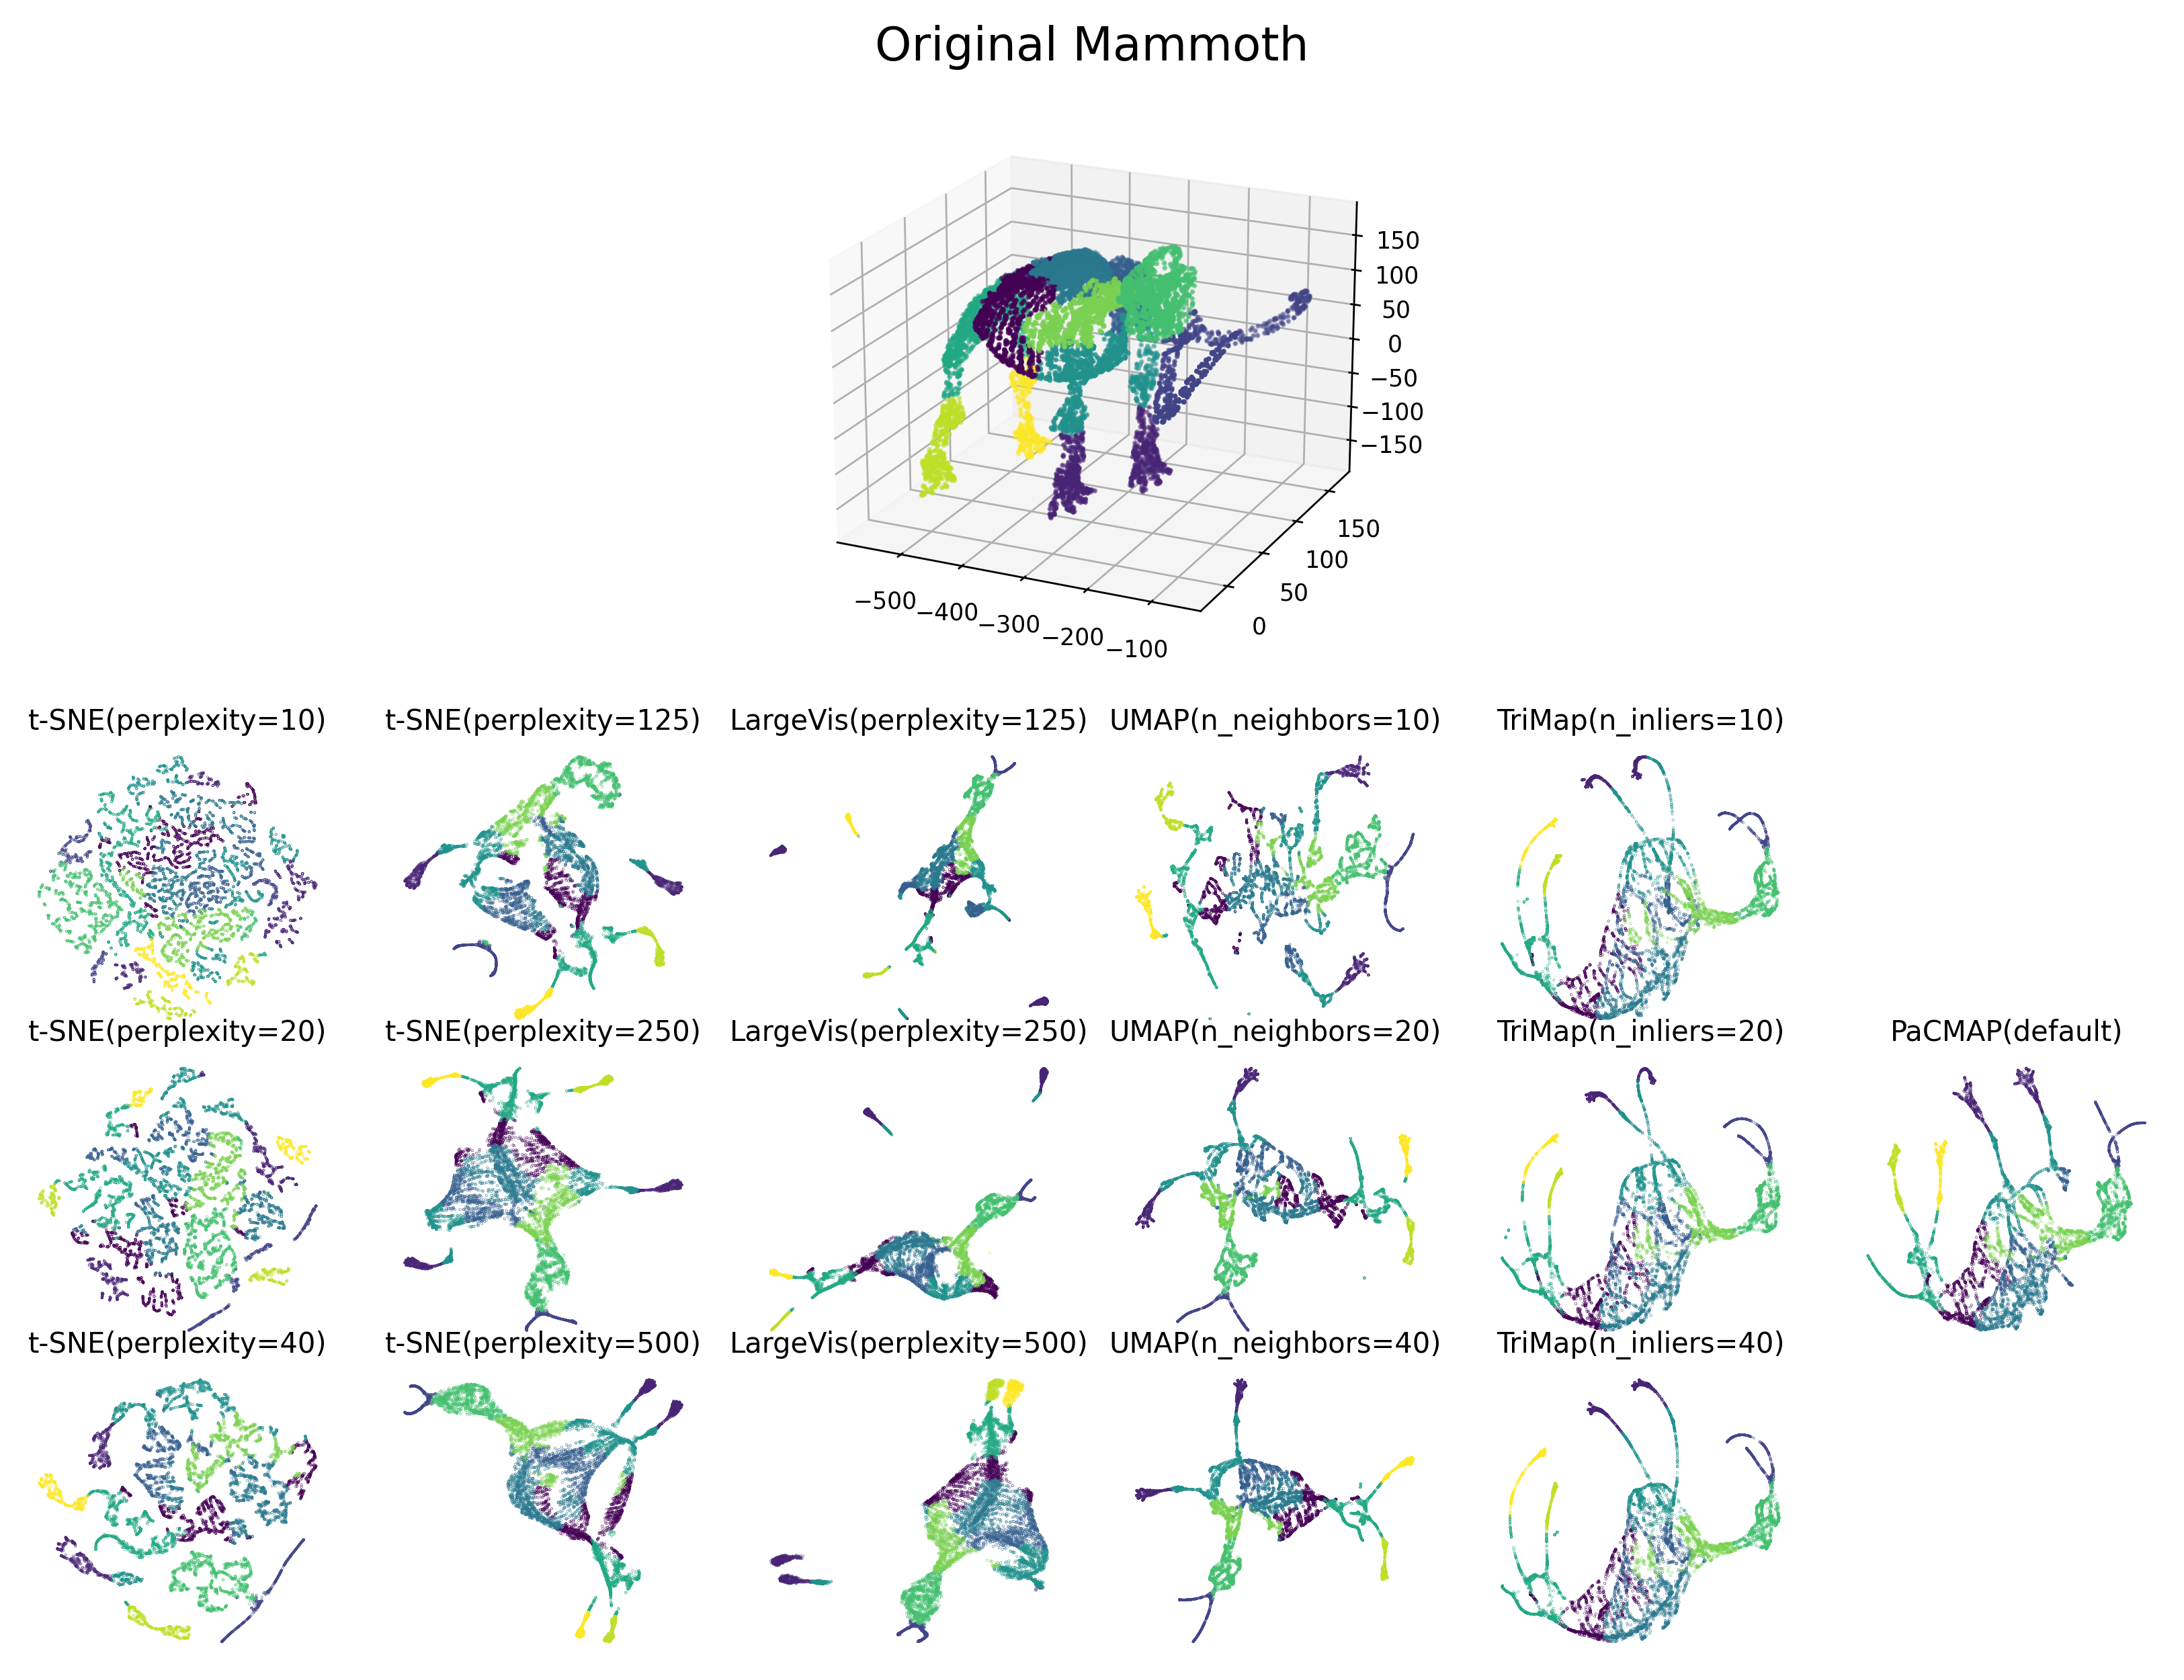
\includegraphics[width=0.95\columnwidth]{figures/Mammoth_21_3}
		\caption{Application of t-SNE, LargeVis, UMAP, TriMAP and PaCMAP to the Mammoth dataset, with their most important parameters shown. The preservation of local versus global structure is clear from looking at small details (such as the toes and tail of the mammoth) and the overall shape of the embedding.}
		\label{fig:Mammoth}
	\end{center}
\end{figure}